\chapter{Foundation}

    \begin{blockquote}
        \paragraph{Intent:} General background information needed to follow the terms and methods used in this thesis.
        
        Structure:
        \begin{description}
            \item[1. Parameter tuning] Parameter tuning of a black-box
                \begin{enumerate}
                    \item $f(Parameter) = Objective$ 
                    \item Goal is optimize $f$
                    \item Problem: Optimization of multiple objectives
                \end{enumerate}
            \item[2. Multi-objective optimization] General definition. Pareto front and None-dominated solution
                \begin{enumerate}
                    \item What is a multi-objective solution?
                    \item How to compare solutions? $\rightarrow$ Types of metrics
                    \item How to solve? $\rightarrow$ Scalarizing, MOEA, Random
                    \item Problem: Reduce evaluations $\rightarrow$ Surrogate optimization, MBMO
                \end{enumerate}
            \item[3. Surrogate optimization] Approach for reducing evaluation count
                \begin{enumerate}
                    \item Intro. Cons and Pons
                    \item Types of a surrogate model in a MO-problem (Model of scalarization, MO-model, Replicated MO-model, Compositional MO-model). Taxonomy
                    \item Surrogate assistance for MO parameter tuning $\rightarrow$ Reusable/scalable components for optimization $\rightarrow$ Problem: Scalability of a surrogate model. [RQ2 \ref{RQ2}]                   
                    \item Surrogate model is domain-specific $\rightarrow$ Analyze multiple surrogates $\rightarrow$ Surrogate portfolio [RQ1 \ref{RQ1}]
                    \item Sampling plan. Build a surrogate model. Quality of prediction depends on the accuracy of a surrogate model  $\rightarrow$ Accuracy depends on a sample size $\rightarrow$ Sample size depends on surface type $\rightarrow$ Problem: Sample size is static. [RQ3 \ref{RQ3}]
                \end{enumerate}
            \item[4. Scope of work] Starting point of thesis
                \begin{enumerate}
                    \item Problem: Expensive black-box with multiple objectives
                    \item Constraint: Evaluation budget
                    \item Goal: Set of MO solutions closed to Pareto-front $\rightarrow$ 1.$Max$ Hypervolume, 2.$Min$ Points-Space, 3.$Max$ \% of None-Dominated points 
                    \item Solution approach: Surrogate model(s) with MOEA
                \end{enumerate}
        \end{description}
    \end{blockquote}

    \paragraph{Intro}
    In this chapter present general background information needed to follow the terms and methods used in this thesis. What is parameter tuning? Why multi-objective is important? Why we can't use the standard multi-objective approach in real-life problem/parameter tuning task, and why model-based or surrogate optimization is the best solution?

    In common old-fashioned software design, engineers carefully convert overall models into domain-specific tools. In this approach, designers codify the current understanding of the problem into the parameters. 

    % --------------------------------------------------------------------------------------------
    % ------------------------------------------------        Parameter tuning
    % --------------------------------------------------------------------------------------------
    \section{Parameter tuning}

        Given recent advances in computing hardware, software analysts either validate engineer models or find optimal configuration by using parameter tuning tools to explore thousands to millions of inputs for their systems. 

        In this article assume that parameter tuning is a subset problem of general, global optimizations. It's also mean that we consider some fitness function $f$ that converts the parameter vector to output objectives.  Note that the term "real evaluation" or "black-box evaluation" as a synonym for the fitness function $f$. 
        
        The goal of parameter tuning as an optimization task lay on fast iterative search with improvements in each objective dimension. The term "fast" means that the convergence to global optimum is achieved with the least real evaluations and shorter time frame.

        We consider fitness function $f$ as black-box with parameter and objective space. Parameter space has structure and could consist from continues and categorical dimensions. Sometimes, some combinations of parameter settings are forbidden. Each point from parameter space lead to some point in objective space. Configurations often yield qualitatively different behavior.
        Objective space also could be described as usual objectives as accuracy, runtime, latency, performance, error rate, energy and so on. On each objective should gain the best possible value and rich system tradeoff.

        Optimization technics:
        \begin{itemize}
            \item Grid search vs Random search
            \item Heuristics and Metaheuristic. (Simulated annealing, Evolutionary algorithm..) These methods aim at generating approximately optimal solutions in a single run. Also could operate with sets of solutions being outcomes of multiple objectives.
            \item Sequential design (Bayesian optimization, Evolutionary algorithm..) Bayesian methods differ from random or grid search in that they use past evaluation results to extrapolate and choose the next values to evaluate. Limit expensive evaluations of the objective function by choosing the next input values based on those that have done well in the past.
        \end{itemize}

        Optimization cost of black-box:
        \begin{itemize}
            \item Evaluation may be very expensive
            \item Sampling budget is unknown
            \item Possibly noisy objectives
            \item Feasibility constraints
            \item Multi-objectivity
        \end{itemize}

        Ideally, we want a method that can explore the search space while also limiting evaluations of hyperparameter choices. 
        The single criterion in parameter tuning may not be sufficient to correctly characterize the behaviour of the configuration space that is why multiple criteria have to be considered.
        One way to clarify the task of understanding the space of possible solutions is to focus on the non-dominated frontier or Pareto-front, the subset of solutions that are not worse than any other but better on at least one goal. The difficulty here is that even the Pareto frontier can be too large to understand. 
    

    % --------------------------------------------------------------------------------------------
    % ------------------------------------------------        Multi-objective       -------------
    % --------------------------------------------------------------------------------------------
    \section{Multi-objective optimization}

        Parameter tuning is present in our daily life and comes in a variety of states. The goal is the rich best possible objective by correctly choosing the system parameters. 
        Common of optimization problems requires the simultaneous optimization of multiple, usually contradictory, objectives. These type of problems are termed as multiobjective optimization problems. The solution to such problems is a family of points, that placing on a Pareto front. Knowledge of the Pareto front allows visualizing appropriate decisions in terms of performance for each objective.

        "Multi-objective optimization(MOO) deals with such conflicting objectives. It provides a
        mathematical framework to arrive at optimal design state which accommodates the various criteria demanded by
        the application. The process of optimizing systematically and simultaneously a collection of objective functions
        are called multi-objective optimization (MOO) \cite{odugod2013}".

        For a multi-objective problem, we consider "solution" as points from parameter space that lead to non-dominated results in objective space. This set of points approximate real Pareto-front. Improving "solution" means that sets of points coincide better with real Pareto-front.

    % ------------------------------------------------        Metrics       -------------
        \subsection{Metrics for multi-objective solution}

        In single-objective minimization, the quality of a given solution is trivial to quantify:
        the smaller the objective function value, the better. However, evaluating the quality of an approximation of a Pareto set is non trivial.
        The question is important for the comparison of algorithms or prediction next configuration.

        According to \cite{ZitzlerDT00}, a Pareto front approximation should satisfy the following:
        \begin{itemize}
            \item The distance between the Pareto front and its approximation should be minimized.
            \item A heigh distribution of the non-dominated points is desirable.
            \item The range of the approximated front should be maximized, i.e., for each objective, a wide range of values should be covered by the non-dominated points.
        \end{itemize}

        Metrics for performance indicators partitioned into four groups according to their properties \cite{Audet2018PerformanceII}: 
        \begin{itemize}
            \item cardinality
            \item convergence
            \item distribution
            \item spread
        \end{itemize}

        Base on the right metrics general multi-objective algorithm keep making progress toward the Pareto front in the objective function space.
        The goal of optimizing a multi-objective problem is to obtain an approximation solution set to the reference Pareto front, including the following subgoals:
        \begin{itemize}
            \item All solution set are as close as possible to the Pareto front
            \item All solution set are as diverse as possible in the objective space
            \item Evaluate as few solution as possible
        \end{itemize}
        Straightforward applying of the simple coefficient of determination (R2) is the wrong indicator of success. Evaluations of different sets of Pareto optimal points is multi-objective task.
        The necessary objectives follow for improving solutions:
        \begin{itemize}
            \item Keep hypervolume low. Reference point is 0 for all objectives.
            \item Maximize sparsity of points. Average distance. Crowding Distance. Spacing metrics.
            \item Maximize non-dominant decisions in the total population
        \end{itemize}

        Also distribution and spread indicators is consider in this work. According to \cite{CustodioMVV11}, “the spread metrics try to measure the extents of the spread achieved in a computed Pareto front approximation”. They are not useful to evaluate the convergence of an algorithm, or at comparing algorithms. They only make sense when the Pareto set is composed of several solutions.

        For multi-objective optimization (MOO), an algorithm should provide a set of solutions that realize the optimal trade-offs between the considered optimization objectives, i.e., Pareto set. Therefore, the performance comparison of MOO algorithms is based on their Pareto sets. In this study, three popular metrics are used to quantify the performance of the algorithms. 
        \begin{itemize}
            \item Hypervolume (HV)\cite{Zitzler2000ComparisonOM}. 
            This metric represents the volume of the objective space that is covered by the individuals of a non-dominated solutions set (solutions that belong to a Pareto front). The volume is delimited by two points: one point that is called the anti-optimal point (A) that is defined as the worst solution inside the objective space, and a second optimal point (pseudo-optimal) that is calculated by the proposed solution method. 
            Determining the hypervolume indicator is a computationally expensive task. Even in case of a reasonably small dimension and low number of points (e.g. 100 points in 10 dimensions), 
            there are currently no known algorithms that can yield the results fast enough for use in most multiple-objective optimizers
            \item Non-dominated Ratio (NDR). This metric employs the non-dominated count of a solution set divided by the total size of solution set. Higher values are preferred to lower ones.
            \item Spacing \cite{Schott1995FaultTD}. Describe the distribution of Pareto points. Fewer space metrics means better coverage of objectives values range.
            
        \end{itemize}

    % ------------------------------------------------        Solving methods       -------------
        \subsection{Solving methods}
        How to search for an optimal solution to the multi-objective optimization problem?
        
            % ----------------      Scalarizing       
            \subsubsection{Scalarizing}
                Scalarizing approach is built on the traditional techniques to creating an alternative problem with a single,
                composite objective function. Single objective optimization techniques are then applied to this composite function to obtain a single optimal solution.
                The weighted-sum methods it's a well known type of scalarizing technic is applied to simplify a multiobjective problem. Concatenate the objectives into one criterion by using magic weighted sum factors. 
                The merged objective is used to evaluate and define the optimal solution.
                Weighted sum methods have difficulties in selecting proper weight especially when there is no connected a priori knowledge among objectives.
                Furthermore, Uniform distribution points in parameters space don't generate uniform distribution points on objective space. This means that we can't approximate Pareto-front completely even with multiple optimization rounds.
                Some scalarizing technics try to improve exploration of parameter space by assigning more "intelligence" aggregation to the objectives. Such solutions may be fragile. They change dramatically if we modify algorithm parameters.

                Moreover, the weighting method can not provide a solution among underparts of the Pareto surface due to “duality gap” for not convex cases. Even for convex cases, for example, in linear cases, even if we want to get a point in the middle of a line segment between two points, we hardly get a peak of Pareto surface, as long as the well-known simplex method is used. This implies that depending on the structure of the problem, the linearly weighted sum can not necessarily provide a solution as DM desires. \cite{Nakayama05}

            % --------------------      MOEA
            \subsubsection{Multi-Objective Evolutionary Algorithms}

                Generating the Pareto set can be computationally expensive and is often infeasible because the complexity of the underlying volume limits exact techniques from being applicable. For this reason, a number of stochastic search strategies such as evolutionary algorithms, tabu search, simulated annealing, and ant colony optimization have been developed: they usually do not guarantee to identify optimal trade-offs but try to find a good approximation, i.e., a set of solutions whose objective vectors are (hopefully) not too far away from the optimal objective vectors \cite{EmmerichD18}.

                The evolutionary algorithm (EA) form a class of heuristic search methods that simulate the process of natural evolution.
                Using simplifications, this EA is subsequently determined by the two basic principles: selection and variation.
                While selection imitates the competition for reproduction and resources among living beings, the other principle, variation, imitates the natural ability to create ”new” living beings through recombination and mutation. Evolutionary algorithm possesses several characteristics that are desirable for problems including multiple conflicting objectives, and large and complicated search spaces. However, EA still need many evaluations of the "black box" system to solve a common multi-objective problem. This is further complicated by the fact that many such problems are very expensive. Consolidated, this makes EAs unfeasible for costly and Multy-objective problem.
                A good solution is the integration of the surrogate model which extrapolate and approximate the fitness landscape from samples. Multi-objective Evolutionary Algorithms (MOEAs) use this surrogate model as a target for optimization. Assumed that solution from surrogate nearby to a global optimum.
                The goal of this thesis is to understand if the performance of MOEAs approach can be improved by using compositional surrogates. The key idea of compositional surrogates is the splitting objective space to multiple surrogates that extrapolate it independently.Combination of multiple hypotheses should give them the potential to approximate more complicated problems. This approach avoids the idea of a single surrogate model, preferring instead to use the composition hypothesis to split out the terrain of objective space.

                The multiple surrogates are analysed on objectives with various complexity, beside the simple and complicated unimodal structure. Generating a cloud of candidates is computationally expensive.

                Evolutionary optimizers explore populations of candidate solutions in each generation, some mutator can make changes to the current population. A select operator then picks the best mutants which are then combined in some way to become generation i+1. 
                This century, there has been much new work on multi-objective evolutionary algorithms with two or three objectives 
                (as well as many-objective optimization, with many more objectives). Multi-objective Evolutionary Algorithms (MOEAs) are popular tools to solve optimization problems, because of their applicability to complex fitness landscapes and solid performance on problems with large design spaces. While other methods also exist, in this thesis we will focus on improving approaches with Evolutionary Algorithms for the Multy-objective optimizations.
                This search-based software engineering is a rapidly expanding area of research and a full survey of that work is 
                beyond the scope of this thesis.

        % ------------------------------------------------        Conclusion       -------------
        \paragraph{Conclusion}
            Motivation for Surrogates

            For optimization expensive black-box:
            \begin{itemize}
                \item Scalable algorithms that convert multi-objective to single objective problem produce solution that not accurate enough(Scalarizing). Also this approach suitable for a limited type of problem. Also, there are a lot important parameters that significant influence on algorithm performance.
                \item Genetic algorithms. This approach is costly to perform and not appropriate for expensive problems.
            \end{itemize}
            Optimization gap in obtaining high quality, multi/single-obj solutions in expensive to evaluate experiments.
            Experiments as a black box, derivative-free. Reference to surrogate optimization.


    % --------------------------------------------------------------------------------------------
    % ------------------------------------------        Surrogate optimization       -------------
    % --------------------------------------------------------------------------------------------
    \section{Surrogate optimization} 

        The potential for applying surrogate is laid in the fast evaluation of the surrogate model. This advantage should outperform disadvantage in time required to build this surrogate model. In classical model-based optimization is used single surrogate-model that provide a hypothesis on the relation between parameter and objective space. There is a lot type of models that can do it but out and away fewer models that can manage multidimensionality objective space. The perspective way to create multi-objective surrogate is stacking multiple simple models into one that describes complex objective space. Notwithstanding that those models could be completely different and build in parallel, they still related because fitted on intersection features.
        Splitting optimization problem to multiple stages improves the reusability of code and makes approach scalable. Nevertheless, we can switch from single-obj to multi obj and change optimization technic on the fly.


        \begin{figure}
            \centering
            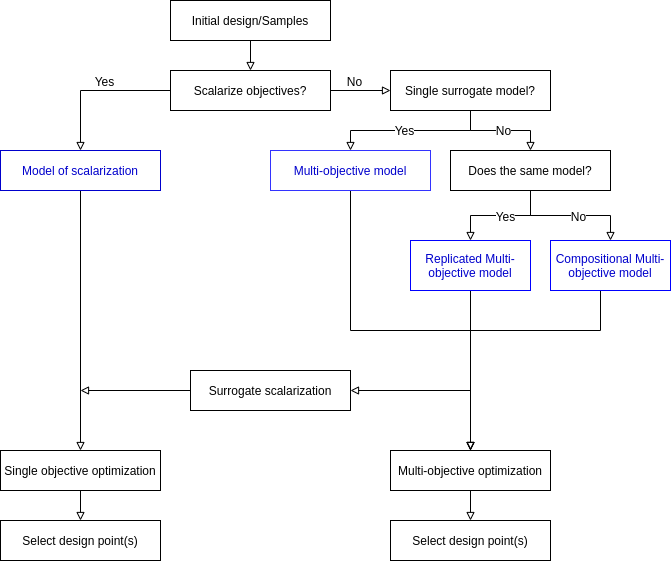
\includegraphics[width=\textwidth]{content/images/mbmo.png}
            \caption[Generalized MBMO algorithm]{Generalized MBMO algorithm}
            \label{fig:generalMBMO}
        \end{figure}


        A surrogate model is either selected randomly or due to its popularity in the area with which the problem is associated.  However, there are still some open challenges related to the ensemble of meta- models such as what should be the criterion for choosing different metamodels or how different metamodels can be used simultaneously? In addition, there are no guidelines for using different models for different objective functions \cite{SoftSurvey}.

        \cite{EngSurMod} 

        To dealing with expensive optimization problem more quickly, we can use surrogate models in the optimization process to approximate the objective functions of the problem. Approximation of solution is faster than the whole optimization process can be accelerated. Nevertheless, the extra time needed to build and update the surrogate models during the optimization process. 
        In the case of pre-selecting the promising individuals, the surrogate model is used to find the likely or drop the low-quality individuals even before they are exactly evaluated, thus reducing the number of exact evaluations.

        In the literature, the term surrogate or model-based optimization is used where, during the optimization processes, some solutions are not evaluated with the original objective function, but are approximated using a model of this function. Different approximation methods are used to build surrogate models. For single and multiobjective optimization similar methods are used. 
        These techniques typically return only one approximated value, which is why in multiobjective problems several models have to be used, so that each model approximates one objective. Some of the most commonly used methods are the Response Surface Method \cite{ResponseSurface}, Radial Basis Function \cite{Rasmussen2004}, Neural Network, Kriging \cite{Woodard00} and Gaussian Process Modeling \cite{RasmussenN10, RasmussenW06}.

        General classification \cite{MlakarPTF15}:
        Within surrogate-model-based optimization algorithms, a mechanism is needed to find a balance between the exact and approximate evaluations. In evolutionary algorithms, this mechanism is called evolution control \cite{Jin05} and can be either fixed or adaptive. In fixed evolution control the number of exact function evaluations that will be performed during the optimization is known in advance. Fixed evolution control can be further divided into generation-based control, where in some generations all solutions are approximated and in the others, they are exactly evaluated \cite{DebN07}, and individual based control, where in every generation some (usually the best) solutions are exactly evaluated and others approximated \cite{Grierson1993}. In adaptive evolution control, the number of exactly evaluated solutions is not known in advance but depends on the accuracy of the model for the given problem. Adaptive evolution control can be used in one of two ways: as a part of a memetic search or to pre-select the promising individuals which are then exactly evaluated \cite{PilatN12}.

        Surrogate used to expedite search for global optimum. Global accuracy of surrogate
        not a priority. Surrogate model is cheaper to evaluate than the objective.

        Bayesian optimization (BO) methods often rely on the assumption that the objective function is well-behaved, but in practice, the objective functions are seldom well-behaved even if noise-free observations can be collected. In \cite{bodin2019modulating} propose robust surrogate models to address the issue by focusing on the well- behaved structure informative for search while ignoring detrimental structure that is challenging to model data efficiently.

        % -------------------------------------------------------------------------------------------------
        % ------------------------------------------------        MO in Parameter tuning       -------------
        \subsubsection{Multi-objective parameter tuning}
        
            % -------------------       Surrogate-model in MOEA       
            \paragraph{Surrogate-model-based MOEA}
            In \cite{KrallMD15} proposed approaches that apply kind of surrogate assistant to evaluations and ranging new population. It allows detecting the most informative examples in population and evaluates them. 
            Identifies and evaluates just those most informative examples at the end done fewer evaluations of the real system. Another way to explore solutions is to apply some heuristic to decompose the total space into many smaller problems, and then use a simpler optimizer for each region. 

            Surrogates are also used to rank and filter out offspring according to Pareto-related indicators like the hypervolume \cite{EmmerichGN06}, or a weighted sum of the objectives \cite{TaboadaBCW07}. The problem with the methods that use hypervolume as a way of finding promising solutions is the calculation time needed to calculate the hypervolume, especially on many objectives. Another possibility is described in \cite{Li2009}, where the authors present an algorithm that calculates only non-dominated solutions or solutions that can, because of variance, become non-dominated. 
            
            GP-DEMO \cite{MlakarPTF15} The algorithm is based on the newly defined relations for comparing solutions under uncertainty. These relations minimize the possibility of wrongly performed comparisons of solutions due to inaccurate 
            surrogate model approximations. Using this confidence interval, we define new dominance relations that take into account 
            this uncertainty and propose a new concept for comparing solutions under uncertainty that requires exact evaluations 
            only in cases where more certainty is needed.


            % ------------------        Surrogate-model with MOEA       
            \paragraph{Surrogate with MOEA}
            Kind of extending the search stage of MOEA with surrogate to simulate evaluation of population. It transform the problem of searching a new better population to improving general hypothesis of how and where Pareto set presented.  

            In surrogate-model-based multiobjective optimization, approximated values are often mistakenly used in the solution comparison. As a consequence, exactly evaluated good solutions can be discarded from the population because they appear to be dominated by the inaccurate and over-optimistic approximations. This can slow the optimization process or even prevent the algorithm from finding the best solutions \cite{MlakarPTF15}. 
            
            % ------------------        Compositional architecture       
            \paragraph{Compositional architecture}
            We could describe compositional-based surrogate optimization as compound grey-box system whit a lot of open research areas where surrogate should improve, managing portfolio, compare of predictions Pareto fronts. 
            As a developer, you can be focused on a specific problem and don't know how to implement other components. This is one of the main advantages of the described approach.
    
            \paragraph{Compositional surrogates}
            Can the same single-objective models be equally applied to various types of problems in multi-/single-objective optimization?
            When there is no correlation between the objectives, a very simple way to solve this kind of problem is to build independent models, i.e. one for each objective, and then to use those models to simultaneously extrapolate possible solutions with MOEA. Nevertheless, the output values correlated, but an often naive way to build multiple models that able to extrapolate complex objective space is often given good results.  
    
            Later research generalized this approach. MOEA/D (multiobjective evolutionary algorithm based on decomposition \cite{ZhangL07}) is a generic framework that decomposes a multi-objective optimization problem into many smaller single problems, then applies a second optimizer to each smaller subproblem, simultaneously.
    
            With multiple models, their flaws can combine, as well as the time required to build the models. In memetic algorithms, especially if the surrogate model is not very accurate, a local optimum can be found instead of the global optimum. But in terms of parameter tuning, this point should be better than a predefined sampling plan. Evaluation of this prediction improve surrogate model quality in the near-optimal area and improve prediction in the next round.
            For example, OEGADO \cite{ChafekarSRX05} creates a surrogate model for each of the objectives. The best solutions in every objective get also approximated on other objectives, which helps with finding trade-off individuals. The best individuals are then exactly evaluated and used to update the models.
        

        % --------------------------------------------------------------------------------------------
        % ------------------------------------------------     Domain-specific Surrogate model      
        \subsection{Domain-specific problem}
        With gain to find the best solution with less effort surrogate models is domain-specific. It's mean that from two surrogate models in two different problems the best surrogate is changing. It could interpreter as Non-free lunch theorem in model-based optimization. If we extend this argument then the same optimization problem in different parameter tuning iteration could be interpreted as another optimization problem. This means that to reduce effort and increase the convergence of an algorithm we should change the surrogate model depend on how much samples do we have. As one would expect, no approximation method is universal.
        This leads us to use a portfolio with surrogate models. As a negative consequence, the model fitting additional introduces an additional overhead into the optimization.


        % --------------------------------------------------------------------------------------------
        % ------------------------------------------------     Build surrogate model     
        \subsection{Build the surrogate model(s). Sampling plan}



        % --------------------------------------------------------------------------------------------
        % -------------------------------------------------------        Discussion       ------------
        \paragraph{Discussion}
        Example of each type of optimization. Justification solution.
        Conclusion: Design gap in optimization/parameter tuning. 
        Need to indicate optimization workflow for expensive process/experiments. 
        The argument(s) why we need a new architecture. Reference to composition architecture.

        Surrogate based optimization has proven effective in many aspects of engineering and in applications where data is "expensive", or difficult, to evaluate.

    % --------------------------------------------------------------------------------------------
    % ------------------------------      Compositional Surrogate optimization       -------------
    % --------------------------------------------------------------------------------------------


    \section{Scope of work}
        \todo{make some nice tree-diagram}

        Describe and implement workflow for multi-objective parameter tuning of the derivative-free, black-box system. Parameter estimation is costly. The proposed solutions are also suitable for single-criteria optimization. Problem Setting.

        Goal:
        \begin{enumerate}
            \item Globally optimize an objective function(s) that is expensive to evaluate. Single/Multi-objective parameter tuning
            \item Simultaneously optimization scalable objectives
            \item Components reuse. Extensibility with other frameworks
        \end{enumerate}

        Problem:
        \begin{enumerate}
            \item A large number of the target black-box evaluations
            \item Interfaces not unify
            \item Code duplication
        \end{enumerate}

        Solution:
        \begin{enumerate}
            \item Component-Based Architecture
            \item Compositional-based surrogate optimization with MOEA
        \end{enumerate}
